
\section{A vortex pair in a thermal field}\label{ch07:field}

\subsection*{The instrument}

The field is the projected Gross--Pitaevskii equation $i\partial_t\psi=\mathcal P[-\tfrac12\nabla^2\psi+g|\psi|^2\psi]$ on a periodic square box of side $L=64$, with $\hbar=m=g=1$ and mean density $n=1$ (healing length $\xi=1$, sound speed $c=1$),
$128\times128$ grid points and a sharp cutoff $|k|\le k_c=\pi$, half the grid wavenumber~\cite{Davis2001,Blakie2008}. The energy is conserved (to $10^{-7}$--$10^{-6}$ over every run of the campaign); nothing is damped and no noise is added. The temperature of a
base state comes from an equipartition thermometer and its normal fraction from the current correlators~\cite{Callens2026a}. The base state of this section is the campaign's $e=0.60$ state: $T=0.115$, that is $T/T_{\rm BKT}=0.14$ with $T_{\rm BKT}(L{=}64)=0.821$ from a heating
ladder, and $\rho_n/\rho=0.027$.

A pair is written into the state by multiplying $\psi$ by the Jacobi-theta phase of the vortex configuration, made single-valued on the torus by a uniform phase gradient, and by the Bernoulli amplitude $[1+|\mathbf v|^2/2]^{-1/2}$ of the imprinted flow. Vortices are found by the
plaquette phase-winding rule that \lean{VortexWinding} proves correct (\cref{ch03}), refined to sub-grid precision, followed by continuity (same sign, nearest detection within $3\xi$) and recorded every time unit. A single pair in a periodic box carries impulse and drives a mean flow, so the
simulations imprint \emph{two antiparallel pairs}, a $+-$ pair at $x=L/4$ and a $-+$ pair at $x=3L/4$ of equal separation $d_0$: zero net charge, dipole moment and impulse, the two pairs travelling in opposite directions.

\begin{rustbox}{two antiparallel pairs in a thermal field (qf-pgpe)}
\begin{lstlisting}[style=py,basicstyle=\ttfamily\footnotesize]
@@BOOKBLOCK{figures/ch07_pairrun.py}{imprint,track,step}@@
\end{lstlisting}
\nopagebreak[4]\smallskip\noindent\textit{Excerpt of \texttt{book/figures/ch07\_pairrun.py}, as run (\texttt{s} is \texttt{qf\_pgpe.Pgpe(128, 64.0)}, \texttt{c} the projected Fourier amplitudes, \texttt{last} the previous positions). The run was advanced in @@RUN_NCHUNK@@ chunks of $@@RUN_CHMIN@@$ to $@@RUN_CHMAX@@$ time units, each under the
shared-machine lock, and checkpointed: @@RUN_SECONDS@@\,s of wall-clock for @@RUN_TEND@@ time units on one thread, at load average @@RUN_LOAD@@ on 8 cores.}
\end{rustbox}

\subsection*{The control that caught the first instrument}

An instrument has to be tested where the answer is known. At $T=0$ a pair in a uniform condensate has no excitation to rub against, and the model says its separation must not shrink. The campaign's first known-answer gate did not use this control: it was a single dipole at $T/T_{\rm BKT}\approx0.14$ with the
imprint of the earlier rounds and a biased vortex detector, and it \emph{passed}, narrowly: four fits gave $\alpha=0.0093,\ 0.0062$ ($d_0=8$) and $0.0028,\ 0.0022$ ($d_0=12$), median $0.0045$, inside the window $[0.004,0.045]$ registered from an interpolation of the values published by Shukla, Brachet and Pandit~\cite{Shukla2014}.
That the friction fell with the size of the pair was not predicted, and was noted. The $T=0$ control was run next, and it failed.

\begin{figure}[!tb]\centering
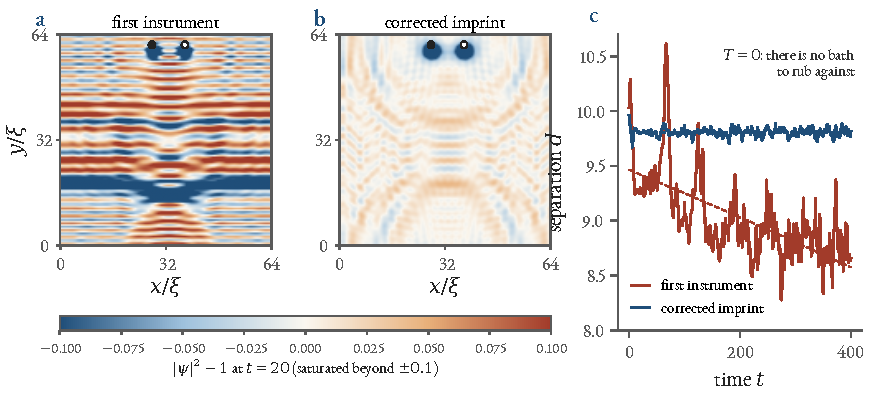
\includegraphics[width=\linewidth]{figures/ch07_imprint.pdf}
\caption[A zero-temperature control of the vortex imprint]{A $T=0$ control. A single pair of separation $10$ is imprinted in a uniform condensate ($L=64$) and $|\psi|^2-1$ is shown $20$ time units later. \textbf{a}~The imprint of the first instrument leaves a phase step along a whole line of the box and a density tail, which become a sheet of sound.
\textbf{b}~The corrected imprint leaves a quiet wake. \textbf{c}~Separation against time over $400$ time units, from the archived tracks of the two gate runs (first attempt: failed; second: passed); dashed, a straight line fitted to $d^2$.}
\label{ch07:fig-imprint}
\end{figure}

\Cref{ch07:fig-imprint} shows why. With the first imprint the pair, which cannot lose energy to a bath that does not exist, closed from $10.03$ to $8.66$ in $400$ time units: an \emph{apparent} friction $\alpha=@@IMP_ALPHA_OLD@@$ from the slope of $d^2$, more than the thermal value measured later at $T/T_{\rm BKT}=0.14$ ($0.0062$).
The peak density just after the imprint is @@IMP_PEAK_OLD@@ against @@IMP_PEAK_NEW@@ with the corrected one, and at $t=20$ the field momentum is @@IMP_MOM_OLD_RATIO@@ of $2\pi nd$ against @@IMP_MOM_NEW_RATIO@@. Two defects were responsible: the theta-function phase of a single pair is periodic on the torus only if
$\sum_iq_i\mathbf r_i\in L\mathbb Z^2$, otherwise it jumps by $2\pi d/L$ across a boundary and the projection turns the jump into a sheet of sound; and the usual per-vortex amplitude $[r^2/(r^2+2)]^{1/2}$ has a $1/r^2$ tail four times the Bernoulli depletion, whose excess leaves as sound and pushes the vortices (cf.~\cite{Rorai2013}).
With the corrected imprint the pair stays at $9.96\to9.81$ ($|\alpha_{\rm apparent}|<10^{-5}$).

The ledger records the consequence without softening: the pass of the first gate \emph{is withdrawn}, and the stalled single pair that had motivated the hypothesis of \cref{ch07:wind} lost its standing as evidence. The replacement is the corrected instrument at $T=0.115$ with a window fixed in advance: $\alpha_{\rm energy}=0.00705\pm0.00012$ in $[0.0028,0.0112]$.
The lesson is which known answer to ask for first: the $T=0$ control is the cheapest, and the one a theorem makes decisive, since with no bath there is nothing to dissipate into.

\subsection*{The field, and what is measured in it}

\begin{figure}[!tb]\centering
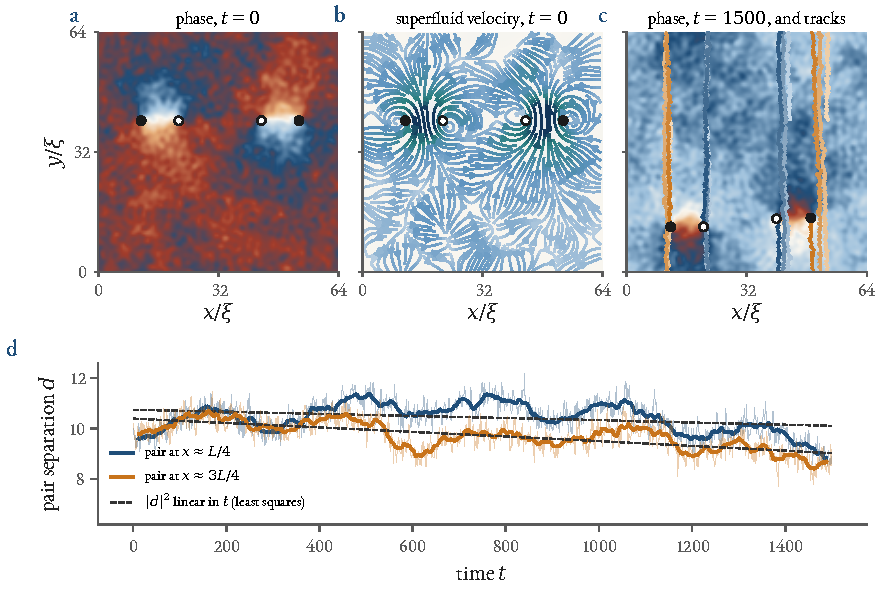
\includegraphics[width=\linewidth]{figures/ch07_fields.pdf}
\caption[Two antiparallel vortex pairs in a thermal projected Gross--Pitaevskii field]{Two antiparallel vortex pairs in a thermal projected-GP field ($T=0.115$, $T/T_{\rm BKT}=0.14$, $L=64$, $d_0=10$), evolved with the Rust engine @@FIELDS_NOTE@@.
\textbf{a}~Phase of $\psi$ just after the imprint; open circles are $+$ vortices, filled circles $-$ vortices. \textbf{b}~The superfluid velocity $\mathrm{Im}(\psi^*\nabla\psi)/|\psi|^2$ coarse-grained over $3\xi$: the jets between the members of each pair and the return flow around them;
the thermal phonons are the faint background. \textbf{c}~Phase at the end of the run with the four tracks (colour: time, drawn on the periodic box). \textbf{d}~Separations of the two pairs against time; dashed, least-squares fits of $d^2$ against $t$.}
\label{ch07:fig-fields}
\end{figure}

\Cref{ch07:fig-fields} shows what the instrument sees. At $t=0$ each pair is a dipole: between its members the superfluid velocity is a jet of speed about $1/d$, the two jets point in opposite directions, and each vortex rides on the jet of its partner. Over @@RUN_TEND@@ time units the two pairs travel about @@RUN_LAPS@@ times round the box in opposite directions, at the speeds @@RUN_SPEEDS@@ (the planar $1/d$ would give about $0.1$). The torus point-vortex model, evaluated at the tracked positions, gives @@RUN_MODEL_SPEEDS@@: the measured speed is @@RUN_SPEED_RATIOS@@ of the model's, the regression coefficient $1-\alpha'$ below being @@RUN_OMA@@ (jackknife over eight blocks of the track), so that the centre moves at the model velocity with no sideways force within the errors, as the centre identity of \cref{ch07:lean} says it should. (The planar formula $1/d$ is @@RUN_PLANAR_LOW@@ per cent below the model for the two pairs: the model adds the periodic images and the second pair.) The separations go from @@RUN_D0@@ to @@RUN_DEND@@, between @@RUN_DMIN@@ and @@RUN_DMAX@@ along the way: the run @@RUN_ENDED_PHRASE@@. The detected position of a core jitters by @@RUN_JIT@@ per coordinate (the zero-lag offset of the residuals, $c_0=@@XCHK_C0@@$, for the archived runs of this arm).
A least-squares slope of $d^2$ reads $\alpha=@@RUN_ALPHA_D2@@$ (mean of the two pairs; separately @@RUN_A1@@ and @@RUN_A2@@): to be compared with the estimators below, not trusted over them.

The estimators the programme registered are the energy identity~\eqref{ch07:eq-energy} and a two-coefficient regression: for each tracked vortex the displacement over a lag of $10$ time units is regressed on $\int\mathbf v_{s,i}\,dt$ and $-q_i\!\int\hat{\mathbf z}\times\mathbf v_{s,i}\,dt$, with $\mathbf v_{s,i}$ the torus point-vortex velocity induced by the \emph{other tracked vortices}; the
coefficients are $1-\alpha'$ and $\alpha$, and the mean square of the residuals against lag gives $\eta$. Both are in the Rust extension, \texttt{qf\_pgpe.analyse\_tracks(tracks, 64.0)}, which takes a list of (times, positions, charges) and returns the estimates with block-jackknife errors. It agrees with the Python code of the campaign to $@@XCHK_RELDIFF@@$ (relative) on the eight archived tracks
of this arm (Python: @@XCHK_PY_S@@\,s; Rust: @@XCHK_RS_S@@\,s, on the loaded machine) and reproduces the campaign's numbers: $\alpha_{\rm energy}=@@ARCH_AE@@\pm@@ARCH_AE_SE@@$, $\alpha_{\rm regression}=@@ARCH_AR@@\pm@@ARCH_AR_SE@@$, $1-\alpha'=@@ARCH_OMA@@\pm@@ARCH_OMA_SE@@$.

\begin{figure}[!tb]\centering
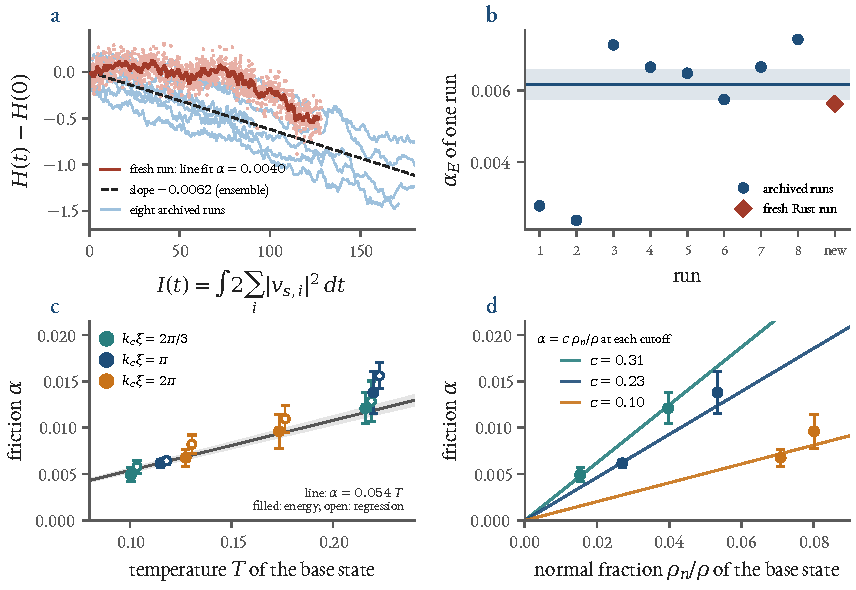
\includegraphics[width=\linewidth]{figures/ch07_friction.pdf}
\caption[The friction in the field]{The friction in the field. \textbf{a}~The energy identity on the tracks: $H(t)-H(0)$ against $I(t)=\int2\sum_i|\mathbf v_{s,i}|^2dt$ falls along a line of slope $-\alpha$ (red: the fresh run, samples and means of $25$ consecutive samples; light blue: the eight archived runs, the same means over the same duration; dashed: the slope of the ensemble).
\textbf{b}~Single-run estimates $\alpha_E$ at $T=0.115$: the eight archived runs and the fresh one, against the ensemble mean and its jackknife error (band). \textbf{c}~The friction of the six arms of the cutoff scan against the temperature of the base state (filled: energy estimator; open, shifted right: regression); the line is
$\alpha=0.054\,T$ (band: one standard error). \textbf{d}~The same data against the normal fraction: within each cutoff the points are proportional to $\rho_n/\rho$, with a coefficient $c$ that changes by a factor $3$ from one cutoff to the next.}
\label{ch07:fig-friction}
\end{figure}

\Cref{ch07:fig-friction}a is the theorem at work, with its caveat. For every run $H(t)$ and $I(t)$ are computed from the tracked positions only, and the identity says that they lie on a line of slope $-\alpha$. The eight archived runs (light blue) do, within the thermal scatter of the detected positions, but with slopes that differ from run to run: over the same
@@RUN_TEND@@ time units their single-run $\alpha_E$ has a mean of $@@SINGLE_MEAN@@$ and a standard deviation of $@@SINGLE_SD@@$, @@SINGLE_CV@@ per cent of the mean (panel~b). The fresh run (red) gives $\alpha_E=@@RUN_AE@@$ and $\alpha_R=@@RUN_AR@@$ from the registered estimators (they fit the two halves of every track separately and pool them, so that block-jackknife errors can be given; one straight line through the whole track gives $@@RUN_AE_DIRECT@@$). That puts the run @@RUN_VERDICT@@.
It is one seed, drawn once and not replaced. The same run analysed at its checkpoint $t=1000$, while the last chunk was waiting for a processor, had given $\alpha_E=@@RUN_AE1000@@$ and $\alpha_R=@@RUN_AR1000@@$: the estimate of one track moved by @@RUN_MOVE@@ in $500$ time units, and nothing was decided on that interim look.
A pair at this temperature should lose $4\alpha t\approx@@RUN_SHRINK@@$ in $d^2$ over the run, that is, $d$ should fall from $10$ to $@@RUN_FALL@@$; but the separation of one pair wanders by @@RUN_DWANDER@@ within the run (\cref{ch07:fig-fields}d), so a single track cannot isolate the drift. That is why the campaign used six to eight runs per temperature and quoted jackknife errors over runs; and it is the reason that the identity,
which is exact in the model, is a way of \emph{estimating} $\alpha$ and not a way of seeing it in one track.

\begin{table}[!tb]\centering\small
\begin{tabular}{lcccccc}
\toprule
$T$ & $T/T_{\rm BKT}$ & $\rho_n/\rho$ & runs & $\alpha$ (energy) & $\alpha$ (regression) & $\alpha_{d_0=8}/\alpha_{d_0=12}$\\
\midrule
$0$ & $0$ & $0$ & 1 & $@@T0_AE@@$ (floor) & $@@T0_AR@@$ & ---\\
$@@E060_T@@$ & $0.14$ & $@@E060_RN@@$ & $@@E060_N@@$ & $@@E060_AE@@\pm@@E060_AE_SE@@$ & $@@E060_AR@@\pm@@E060_AR_SE@@$ & $@@E060_RATIO@@$\\
$@@E070_T@@$ & $0.27$ & $@@E070_RN@@$ & $@@E070_N@@$ & $@@E070_AE@@\pm@@E070_AE_SE@@$ & $@@E070_AR@@\pm@@E070_AR_SE@@$ & $@@E070_RATIO@@$\\
$@@E080_T@@^{\dagger}$ & $0.43$ & $@@E080_RN@@$ & $@@E080_N@@$ & $@@E080_AE@@\pm@@E080_AE_SE@@$ & $@@E080_AR@@\pm@@E080_AR_SE@@$ & $@@E080_RATIO@@$\\
\bottomrule
\end{tabular}
\caption{Friction of a vortex pair in the closed field ($L=64$, $k_c=\pi$; two antiparallel pairs of sizes $8$ and $12$, tracks of up to $2000$ time units), the archived campaign re-analysed with the Rust estimators. Errors are block jackknives over runs.
$^\dagger$A thermal vortex is present in more than $5\%$ of the samples of this base state; the error is large and the base is kept with that flag. The energy estimator is low by the diffusion bias of \cref{ch07:bias}.}
\label{ch07:tab-alpha}
\end{table}

\Cref{ch07:tab-alpha} gives the friction at the three temperatures. The three criteria registered for it passed: the two pair sizes agree (ratios $@@E060_RATIO@@$, $@@E070_RATIO@@$, $@@E080_RATIO@@$, inside the registered $[0.7,1.43]$ at two of three temperatures), $\alpha$ increases with
$T$, and the two estimators agree within $5$, $13$ and $18$ per cent. At $0.14\,T_{\rm BKT}$ the value is a factor two below an interpolation of the values of Shukla, Brachet and Pandit~\cite{Shukla2014}, whose own transition temperature is an estimate; at $0.27$ and $0.43$ no closed-field value existed before, and these lie in the range of the oblate-condensate
measurements~\cite{Moon2015}. One more observation was \emph{not} registered, and is the subject of the next section: $\alpha/(\rho_n/\rho)=0.23,\,0.26,\,0.22$.

\section{Friction follows the temperature, not the normal density}\label{ch07:law}

\subsection*{A kinetic reading, a proportionality, and a prediction}

In the projected field the bath is a finite set of modes $k\in K$ (@@MODES_PI@@ of them at $k_c=\pi$ in this box). For excitations of occupation $n_k$ and transport cross-section $\sigma_{\rm tr}(k)$ (a length, in two dimensions), a vortex moving slowly through them feels the drag $F=-Dv$ with
$D=\tfrac12\int\frac{d^2k}{(2\pi)^2}(-\partial n/\partial\varepsilon)\,k^2\,c_g\sigma_{\rm tr}$, $c_g=d\varepsilon/dk$, while the Landau normal density of the same gas is $\rho_n=\tfrac12\int\frac{d^2k}{(2\pi)^2}(-\partial n/\partial\varepsilon)\,k^2$: two integrals of the same weight, the first with one extra factor $c_g\sigma_{\rm tr}$.
A force balance on a weakly damped vortex gives $\alpha=D/(\rho_s\kappa)$. The finite sums are what Lean sees: with nonnegative weights $w_k$ and drag factors $f_k=c_g\sigma_{\rm tr}$, $D=\sum_kw_kf_k$ and $\rho_n=\sum_kw_k$, so that $\alpha/(\rho_n/\rho)$ is $\rho/(\rho_s\kappa)$ times the $w$-weighted mean of $f$, and that mean lies between the smallest and the largest $f$ over the bath.

\begin{leanbox}[unbreakable]{FrictionKinetic}
\begin{lstlisting}[style=lean,basicstyle=\ttfamily\footnotesize]
@@LEAN{FrictionKinetic.lean}{30-30}@@

@@LEAN{FrictionKinetic.lean}{32-33}@@

@@LEAN{FrictionKinetic.lean}{35-36}@@

@@LEAN{FrictionKinetic.lean}{40-41}@@

@@LEAN{FrictionKinetic.lean}{46-48}@@
\end{lstlisting}
\nopagebreak[4]\smallskip\noindent\textit{Statements only; the proofs are in the module.}
\end{leanbox}

The two theorems are \Lthm{FrictionKinetic}{coeff_eq_weighted_mean} and \Lthm{FrictionKinetic}{weighted_mean_mem_Icc}; for a Rayleigh--Jeans bath with phonon dispersion the weights are equal (\Lthm{FrictionKinetic}{rayleigh_jeans_mean}). Two things follow, and the programme drew only the first. The law $\alpha\propto\rho_n$ is an
\emph{identity} of the kinetic model, for any bath. And its coefficient is not a number about the vortex: it is a mean of $c_g\sigma_{\rm tr}$ \emph{over the modes of the bath}. The module says so itself: ``No claim about the value or the $k$-dependence of $\sigma_{\rm tr}$ is made; that is the measurement.''

At $k_c=\pi$ the measurement gave $\alpha/(\rho_n/\rho)=0.23,\,0.26,\,0.22$ over a factor $3.5$ in $\rho_n$, and the first paper read that coefficient as the mode-averaged transport cross-section of the vortex, $\approx1.4\xi$, ``the geometric size of the core''~\cite{Callens2026a}. That reading assumes that the coefficient belongs to the vortex and not to the bath; the check is to change the bath. The programme registered the test before running it, at two further
cutoffs ($k_c=2\pi/3$ and $2\pi$, same instrument, $T=0$ known answer reproduced at each): FL2, the coefficient differs between the three cutoffs by less than $20\%$, as a property of the vortex should; against a rival, the Born law of long-wavelength phonon scattering extended to the cutoff, which makes it proportional to $k_c$ ($0.67:1:2$).

\subsection*{Both predictions fail}

The coefficient is $@@C_23@@\pm@@C_23_SE@@$, $@@C_31@@\pm@@C_31_SE@@$ and $@@C_63@@\pm@@C_63_SE@@$ at $k_c\xi=2.1,\ 3.1,\ 6.3$ (weighted means over the arms of each cutoff, recomputed here from the six arms): the spread $(\max-\min)/\text{mean}$ is $@@C_SPREAD@@$ against the registered $0.2$, so FL2 fails; the Born rival fails too ($\chi^2=@@BORN_CHI2@@$ for $2$ degrees of freedom: the
coefficient \emph{falls} with the cutoff, and the Born law makes it rise); one common coefficient for the six arms fails ($\chi^2=@@ONEC_CHI2@@$ for $5$). Proportionality to $\rho_n$ holds within each cutoff where two temperatures exist, as the identity says it must. The implied mode-averaged cross-section $c\,\kappa\,\rho_s/\rho$ is $1.9\xi$, $1.4\xi$ and $0.59\xi$ (ledger values, each arm's own $\rho_s$): not a property of the vortex.
The ``geometric core size'' reading is \textbf{withdrawn}.

What does not move with the cutoff is the friction itself. \Cref{ch07:fig-friction}c shows the six arms on one line, $\alpha/T=@@AT_E@@\pm@@AT_E_SE@@$ ($\chi^2=@@AT_E_CHI2@@$ for $5$ degrees of freedom, against $@@ONEC_CHI2@@$ for a common $c$), or $@@AT_R@@\pm@@AT_R_SE@@$ with the regression estimator ($\chi^2=@@AT_R_CHI2@@$). In the first paper the three temperatures were taken at one cutoff, where
$\rho_n/\rho$ grows in proportion to $T$, so that a proportionality to either could not be told from the other; the cutoff scan broke the degeneracy (\cref{ch07:fig-friction}c,d). The temperature law was found \emph{after} the data of five arms were read. It was registered, as amendment FL-A1, as a hypothesis, with its prediction for the arm still running fixed in advance: $\alpha=0.0094\pm0.0010$ at
$k_c=2\pi$, $T=0.173$, against $0.0077$ if the friction followed $\rho_n$ with that cutoff's coefficient. The arm gave $0.0096\pm0.0018$: inside the window registered for the temperature law, outside the other. The honest reading is smaller than the verdict: the error is almost twice the one assumed when the window was written, so the ledger puts this arm alone at $0.2\sigma$ from one value and $1.0\sigma$ from the other, and the
discrimination rests on the comparison across cutoffs. The law has been tested over $T=0.10$--$0.22$ and three cutoffs, in one box at one coupling; not above $T=0.22$, where thermal vortices enter.

\subsection*{What transfers, and what does not}

LL-15, the programme's rule, says that an analogy between two systems is not a result: name the property a finding depends on and check that the other system has it. The law $\alpha\propto T$ depends on a property of the \emph{bath}. In a classical field every mode carries the energy $T$, so $n_k=T/\varepsilon_k$ and anything linear in the occupation is linear in $T$; if
$\int^\infty\sigma_{\rm tr}\,dk$ converges (for $k\xi\gg1$ the weight of $D$ makes the integrand $\propto\sigma_{\rm tr}(k)$), the friction is also independent of the cutoff, while $\rho_n$ grows logarithmically with it. Does a quantum gas have the property? We computed Landau's formula $\rho_n=\tfrac12L^{-2}\sum_kk^2(-\partial n/\partial\varepsilon)$ for free Bogoliubov quasiparticles, $\varepsilon_k^2=k^2+k^4/4$, on the actual mode set of each of the six arms (\texttt{figures/ch07\_bath.py}), once with the equipartition occupation $n_k=T/\varepsilon_k$ of the field and once with the Bose occupation $1/(e^{\varepsilon_k/T}-1)$ of a gas at the same temperature. The equipartition sum gives @@BATH_FRAC_MIN@@--@@BATH_FRAC_MAX@@ per cent of the measured normal fraction of the arm (the rest is interaction); the Bose sum is smaller than the equipartition one by a factor @@BATH_RATIO_MIN@@ to @@BATH_RATIO_MAX@@.

So the field does not have it. At $T=0.115$ the equipartition occupation of the mode at the cutoff, $k=\pi$ with $\varepsilon=5.85=51\,T$, is $0.020$ and the Bose occupation is $8\times10^{-23}$; at $k=1$ the ratio is @@OCC_RATIO_K1@@; only at $k\lesssim0.2$, $\varepsilon\approx1.75\,T$, do the two agree within a factor $3$. Of the equipartition Landau sum at $k_c=\pi$, $T=0.115$, only
@@FRAC_EPS_LT_T@@ comes from modes with $\varepsilon<T$ ($@@FRAC_EPS_LT_3T@@$ from $\varepsilon<3T$): the normal density of the classical field is carried by modes that a quantum gas at that temperature would not populate, and its normal fraction is about thirty times that of the Bose bath ($0.0227$ against $0.00075$). So the temperature of the classical field is a parameter of the model, which maps onto a physical
temperature only through the cutoff~\cite{Callens2026b}, and the friction law of this section is a law of \emph{this} model; the earlier advice to compare with quantum gases at equal $\rho_n/\rho$ rather than at equal $T/T_c$ is withdrawn in the same sense. What a quantum bath would give, for helium, needs the excitation energies that Godfrin's neutron measurements fix and the cross-section of a vortex for those excitations,
which this programme has not measured. The direct measurement, a monochromatic Bogoliubov wave scattered by one vortex at $T=0$, is the obvious next experiment; it is not in this chapter.
